\documentclass[sigconf, 9pt]{acmart}


\usepackage{xcolor}

\usepackage{float}
\usepackage{siunitx}


\newif\iffinal

% \finaltrue

\iffinal
  \newcommand{\tyler}[1]{}
  \newcommand{\ian}[1]{}
  \newcommand{\kyle}[1]{}
\else
  \newcommand{\tyler}[1]{{\textcolor{cyan}{ tyler: #1 }}}
  \newcommand{\ian}[1]{{\textcolor{red}{ Ian: #1 }}}
  \newcommand{\kyle}[1]{{\textcolor{purple}{ Kyle: #1 }}}
\fi


%%
%% \BibTeX command to typeset BibTeX logo in the docs
\AtBeginDocument{%
  \providecommand\BibTeX{{%
    \normalfont B\kern-0.5em{\scshape i\kern-0.25em b}\kern-0.8em\TeX}}}


\newcommand{\name}{Xtract}
\newcommand{\funcx}{$f$\kern-0.18em\emph{unc}\kern-0.05em X}

\acmConference{Fifth International Workshop on Serverless Computing (WoSC)}{2019}{Davis, CA}

\begin{document}


\title{Harnessing Serverless to Extract File Metadata at the Edge}


\author{Tyler J. Skluzacek} 
\affiliation{University of Chicago}
\email{skluzacek@uchicago.edu}



\renewcommand{\shortauthors}{Skluzacek et al.}

\begin{abstract}
\tyler{max 100 words}

%\tyler{GRAND-er. be more dramatic. }
%\kyle{Maybe here you could say. Lots of data. Its created and stored in different places. 
%We need to rethink the siloed and antiquated file system approach and instead think
%of data in one global index of metadata (i.e., a data ocean -- just made up this term, not sure
%if I like it). To do this we need to be able extract metadata
%from where data exists. We propose a fluid, serverless middleware in which extractors
%are dynamically determined and executed wherever it makes most
%sense (e.g., at the edge, cloud, computing center, ...)}



The rapid generation of data from IoT devices, scientific instruments, and user edge devices presents
unique challenges in data management. Currently these data are distributed and generally siloed, 
but the current capabilities of file systems do not enable users to search these distributed data collections.
 In this work we propose \name{}, a serverless middleware 
that extracts metadata from files on heterogeneous edge computing resources, and conducting the extraction 
where it makes the most sense, whether on the device itself, in the cloud, or on a dedicated cluster. 
To this end, we intend to create a searchable global index across a user's or multiple users' data collections.  
	
	
%In this work
%we propose a middleware architecture called Xtract that leverages serverless 
%computing to simultaneously extract metadata across a continuum of heterogeneous edge 
%devices, from IoT to HPC to 
%laptops. Xtract will enable the curation of an atomic multi-site data lake in which the
%resources can make intelligently scale and move data in order to optimize for various 
%SLAs.


\end{abstract}

\begin{CCSXML}
<ccs2012>
<concept>
<concept_id>10002951.10003227.10010926</concept_id>
<concept_desc>Information systems~Computing platforms</concept_desc>
<concept_significance>500</concept_significance>
</concept>
<concept>
<concept_id>10002951.10003317.10003365.10003366</concept_id>
<concept_desc>Information systems~Search engine indexing</concept_desc>
<concept_significance>300</concept_significance>
</concept>
<concept>
<concept_id>10002951.10003317.10003318.10003319</concept_id>
<concept_desc>Information systems~Document structure</concept_desc>
<concept_significance>100</concept_significance>
</concept>
<concept>
<concept_id>10010405.10010497.10010500.10010503</concept_id>
<concept_desc>Applied computing~Document metadata</concept_desc>
<concept_significance>500</concept_significance>
</concept>
</ccs2012>
\end{CCSXML}

\ccsdesc[500]{Information systems~Computing platforms}
\ccsdesc[500]{Applied computing~Document metadata}
\ccsdesc[300]{Information systems~Search engine indexing}
\ccsdesc[100]{Information systems~Document structure}

\keywords{data lakes, serverless, metadata extraction, file systems, materials science}

\maketitle


\section{Introduction}

The rapid generation of data from IoT devices, scientific instruments, and personal computing devices presents unique 
data management challenges. Currently data are spread across multiple machines, are generally siloed, and require 
significant manual labor by users to create metadata that make the data on these devices searchable. Some~\cite{egan2003vizier, welter2013nhgri, irods, dataverse}  have created data catalogs from user-submitted metadata. These, however, are not scalable to current and future storage systems,
%science and enterprise 
%exascale use cases, 
as humans cannot possibly label billions of heterogeneous files. 
 %spanning exabytes and beyond
%that would be expensive (or outright impossible) to transfer, stage, and process on small cluster file systems and personal computing devices.  
In order to build a global metadata catalog over distributed big data, we require automated methods to crawl data, extract 
metadata attributes for each file, and populate a global search index for users to find and access data. Others have developed end-to-end 
automated metadata extraction systems, but they require that data be moved to a central service~\cite{skluzacek2018skluma, skluzacek2016klimatic, padhy2015brown, rodrigo2018sciencesearch} or must be manually deployed at data~\cite{mattmann2011tika}. 
In this work we strive to create a decentralized metadata extraction system that mitigates the need to send files to a central service.  

%Serverless computing abstracts computing resources from the user, enabling
%the deployment of applications without consideration for the physical and virtual infrastructure on which 
%they are hosted. FaaS allows users to register programming functions with predefined input signatures.
%Registered functions can subsequently be invoked many times
%without the need to provision or scale any infrastructure.

%\kyle{This paragraph repeats some of the previous one. I would vote to remove the previous paragraph}
%\tyler{unplagiarize the first 3 sentences here}
We propose \name{}
a serverless middleware that provides high-throughput and on-demand metadata 
extraction that enables the automated creation of rich, searchable data lakes from previously unsearchable data swamps. 
Serverless computing, and specifically function as a service (FaaS),
provides an ideal model for managing the invocation of
many short-running extractors on an arbitrarily large number of files. 
\name{} uses the \funcx{} serverless supercomputing platform~\cite{chard2019serverless}
to execute functions across diverse and distributed computing infrastructure.
%We propose the use of FaaS for mapping the metadata extraction problem to a 
%collection of granular metadata extractor functions. 
%We describe how such a model can support the flexibility, scalability, and extensibility required
%for scientific metadata extraction. 
Rather than rely on commercial FaaS systems, we explore a novel distributed FaaS model 
that overcomes the limitation of moving large amounts of data to the cloud. 
Instead, we are able to push
metadata extractors to the edge systems on which the scientific data reside. 
The contributions of \name{} are the following: 
%\name{} is advantageous to existing metadata extraction systems in that it: 
\begin{itemize}
\item Is infinitely scalable across all various resource types from clouds to clusters. 
\item Deploy endpoints at data, allowing for the decentralization of data processing. 
\item Present a novel method for automatically constructing unique metadata extractor pipelines for diverse file types. 
\item Intelligently makes data staging decisions based on available resources across all of a user's compute allocations. %\kyle{what is meant by all allocations?}
\item Enable users to submit custom extractor function-runtime pairs that supplement a suite of user supplied extractors.
\item Automatically populates a search index of rich, searchable metadata. 
\item Utilizes secure authentication protocols for data privacy and data sharing across multiple users. 
\end{itemize}

%\kyle{I'd like to see more about the novelty of the assembled pipelines in this list}


The remainder of this paper is organized as follows. 
\S\ref{sec:approach} presents our proposed architecture for \name{}. 
\S\ref{sec:eval} discusses metrics and workloads used to evaluate its performance. 
Finally, \S\ref{sec:conc} contains concluding remarks.


\section{Approach}
\label{sec:approach}

\name{} is a serverless metadata extraction middleware that runs atop the \funcx{} serverless 
computing platform, allowing users to optimize metadata extraction workflows subject to 
extraction time, cost, available compute allocations, and security policies. % (e.g., HIPAA). %KC prob best not to mention HIPAA.
The remainder 
of this section outlines the various components of the system. The \name{} architecture is shown in Figure~\ref{fig:arch}.

\textbf{Metadata extractors} are functions that input a file or group of files, and output a metadata dictionary. 
Each metadata extractor runs in a given runtime \kyle{runtime not defined}, or a container with all the required dependencies (i.e., files or 
libraries) for the extractor to execute.  Our system currently provides a number of built-in extractors, including
those to extract metadata from tabular, structured JSON- or XML-like, free text, and images. In future we work, 
we plan to support user-submitted metadata extractors, automatically generate runtimes based on inferred 
dependency requirements, and also train \name{} to recognize when a user-submitted extractor 
is appropriate for an arbitrary file. 

The \textbf{\name{} service} dynamically applies a set of metadata extractors to files. 
It does so by constructing a dynamic extractor workflows for each file 
or group of files in a repository.  
First, \name{} sends a crawler function to each endpoint specified by the user.  The crawler creates an 
initial metadata dictionary for each file by finding the paths and physical properties (e.g., size, extension, hash) of each file or group of files
in a given data set.  Once the initial dictionary is created, \name{} invokes a file type extractor on each file that determines probable downstream extractors for each file. We've shown in past work~\cite{skluzacek2018skluma} that feeding the first 512 bytes of a file into 
a trained random forests model can predict a file's type with accuracy higher than the Unix `file' command (footnote why? \kyle{does this use magic bits?}) and in less time
than trying and failing random extractors on a given file. Once a file type is determined the extractor executes the remaining library of extractors 
on each file by sending extractor functions to the endpoint, and sending additional extractors based on the returned metadata.  For instance, 
a tabular data file with multiple lines of free text header (e.g., describing experimental setup) may be identified by the system as a tabular file, but 
the metadata from the tabular 
extractor will state the lines of the file that may be eligible for processing by a free text extractor (e.g., extract keywords from it).
Requests to the web service are protected using Globus Auth~\cite{tuecke2016globus}, and all resulting metadata are stored to a searchable Globus Search index. 

\funcx{} \textbf{endpoints} can be deployed across myriad compute providers, from personal computing devices (i.e., laptops), compatible 
IoT devices, cloud providers, and HPC systems.  Endpoints build upon the Parsl~\cite{babuji2019parsl} parallel programming library to 
provision compute resources on a given system, and to manage the execution of functions in containers on said resources. \funcx{} enables 
\name{} to execute metadata extraction functions at any registered and accessible \funcx{} endpoint.  \funcx{} enables \name{} to reliably 
scale to thousands of nodes and simultaneously deploy metadata extraction tasks on arbitrary compute resources. 
\funcx{} supports Singularity and Shifter, allowing \name{} extractors to be executed
on various high performance computing systems. 

\kyle{Maybe the following paragraph should be moved to a future work? We should think 
about how to structure this.  Should we make this more of a complete vision and then outline
our prototype? Or outline our prototype and then describe where its going?} 
Moreover, we 
plan for \name{} to make data staging and resource provisioning decisions subject to a number of user-defined, real-world computing constraints. For instance, 
perhaps in some cases there could exist an idle resource and transferring some data to a different edge device or HPC center could hasten 
the overall execution time.  Perhaps we want to make data staging and allocation decisions that optimize for cost, so \name{} opts to transfer 
data to cheaper (albeit likely slower or smaller) allocations for extraction.  Or perhaps certain data are subject to HIPAA, so we want to keep 
those data on a VPC, but we can stage other data elsewhere to increase extraction performance. 

\begin{figure}[t]
	\centering
	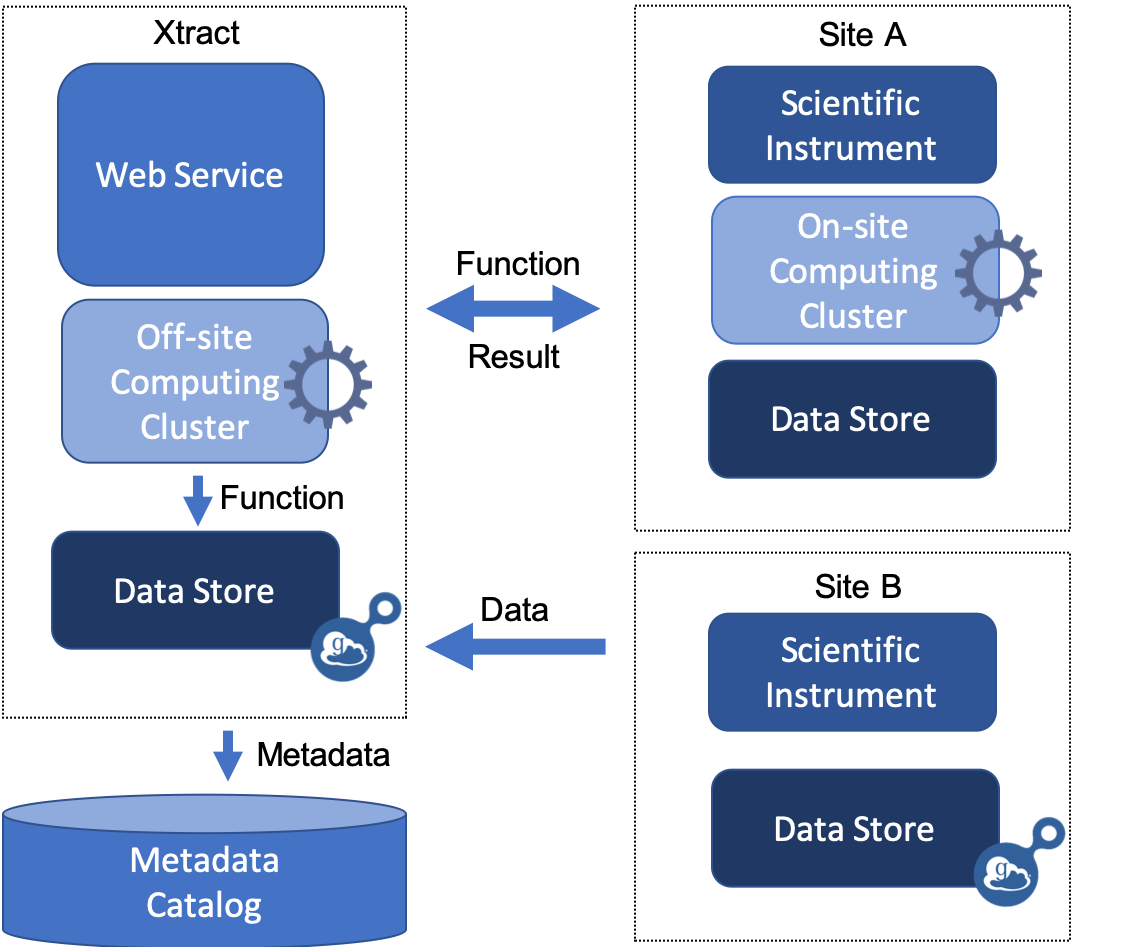
\includegraphics[scale=0.2]{figs/new-arch.png}
	\caption{Overview of the \name{} architecture. For \textit{Site A} functions are transmitted to the remote resource and performed on local computing resources, returning metadata to the \name{} service. \textit{Site B} lacks suitable local
	computing capabilities, requiring data to be staged to \name{} for analysis.}
	\label{fig:arch}
\end{figure}

\name{} implements a comprehensive security model using Globus Auth~\cite{tuecke2016globus}. 
%All interactions with the \name{} Web service are secured with Globus Auth. 
%Users can authenticate with \name{} using one of 
%several hundred identity providers, including many institutions. 
%\name{} uses Globus Auth OAuth~2 flows to stage data on behalf
%of authenticated users. \name{} first verifies a user identity, requests an access
%token to perform data transfers on their behalf, and then uses Globus to stage
%data from remote storage to the \name{} extractor. 
%Finally, the resulting metadata are published into the search index using a Globus Search
%access token. The search index is configured with a \textit{visible\_to} field, restricting
%discovery to authenticated users.


\section{Evaluation Plan}
\label{sec:eval}

We intend to index real science use cases, particularly those in which individual data files are heterogeneous 
or geographically distributed. For each, we intend to explore how to optimize the system across dimensions of 
total compute time (SLAs), monetary cost, security requirements, and resource availability.  We intend to evaluate 
all such dimensions on a diversity of datasets, including the Carbon Dioxide Information Analysis Center (330+ GB, 10,000 
unique file extensions of carbon dioxide data), the Materials Data Facility~\cite{ blaiszik2019mdf} (30+ TB, tens of millions of materials science files); 
Petrel (4+ PB, 50,000+ files of cross-disciplinary data at Argonne National Lab), and Globus (over 20,000 unique, connected 
endpoints containing hundreds of millions of files). \tyler{fact check Globus}

%The Materials Data Facility~\cite{blaiszik2016materials, blaiszik2019mdf}
%is a centralized hub for publishing, sharing, and discovering materials science data. 
%The MDF stores many terabytes of data from many different research groups, covering many disciplines of 
%materials science, and with a diverse range of file types.
%The downside of the expansive range of materials data held by the MDF 
%is that it can be difficult for users to find data relevant to their science.
%The MDF reduces the ``data discovery" challenge by hosting a search index that provides access to metadata from the 
%files (e.g., which material was simulated in a certain calculation).
%
%Petrel? Running out of room. 
%
%Globus~\cite{ananthakrishnan2018globus} manages petabytes of files over tens of thousands of individual user endpoints between research labs, 
%universities, industry, and home computing devices. Many \tyler{???} users elect to have all or part of their data publicly 
%shared with the rest of the Globus community. \kyle{private sharing could also be indexed} Xtract lends itself well to Globus as Globus already deploys an 
%endpoint on the compute node.  We intend to deploy the funcX endpoint as part of the Globus endpoint software, and 
%execute secure metadata extraction over all available petabytes. Globus is particularly useful in studying multi-site 
%metadata extraction, as users generally have multiple active endpoints. \tyler{more detail}. 



\section{Conclusion}
\label{sec:conc}

Metadata extraction at the edge will make previously siloed data searchable and usable by researchers, 
industries with cumbersome data scales, and individuals simply wanting a centralized index across 
each of their files. 


\begin{acks}

This research is conducted under the guidance of Dr. Ian Foster and Dr. Kyle Chard of the 
University of Chicago and Argonne National Lab. This work is made possible in part by the contributions
of Ryan Chard, Yadu N. Babuji, Zhuozhao Li, and Ryan Wong. 


\end{acks}
\bibliographystyle{ACM-Reference-Format}
\bibliography{wosc}


\end{document}
\endinput
